\documentclass[doublecol]{epl2}
%  \documentclass{epl2}
%------reference style ------------------------------
% \usepackage{natbib}
%---------include graphics and maths packages--------
% 	\usepackage{graphicx}
% 	\usepackage{graphics,epsfig}
% 	\usepackage{amssymb}
% 	\usepackage{mathrsfs}
 	\usepackage{amsmath}
% 	\usepackage{color}

\usepackage{psfrag}
%----- definition for figres ------------------------
\def\figdir{./}
%
% %--------- Short hand ---------
%
%
% %------------- Definition of line types --------
% \def\lline{\vrule width12pt height2.5pt depth -2pt}
% \def\mline{\vrule width4pt height2.5pt depth -2pt}
% \def\thmline{\vrule width4pt height3.5pt depth -2pt}
% \def\sline{\vrule width1pt height2.5pt depth -2pt}
% \def\bdot{\raise.2em\hbox to .15em{.}}
% \def\dashed{\mline\hskip4.5pt\mline\hskip4.5pt\mline\thinspace}
% \def\chaindot{\lline\ \bdot\ \lline\thinspace}
% \def\dotted{\bdot\ \bdot\ \bdot\ \bdot\thinspace}
% \def\chaindash{\lline\ \mline\ \lline\thinspace}
% \def\chaindashdash{\lline\ \bdot\ \bdot\ \lline\thinspace}
% \def\solid{\vrule width20pt height2.5pt depth -2pt\thinspace}
% \def\thicksolid{\vrule width20pt height3.5pt depth -2pt\thinspace}
% \def\thickdashed{\thmline\hskip4.5pt\thmline\hskip4.5pt\thmline\thinspace}
%---------- End of definition of line types ------

%---------- Comment block  ------
\long\def\comment#1{}

%---------- Bullet  ------
\def\blt{\hspace*{0.3truein} \noindent --~~}
\def\bblt{\hspace*{0.6truein} \noindent --~~}
\def\nxtln{\hspace*{0.75truein} \noindent}

%----Indentation -------
\setlength{\parindent}{0in}

%----------define indentation for a para --------
\newenvironment{indentpar}[1]%
{\begin{list}{}%
         {\setlength{\leftmargin}{#1}}%
         \item[]%
}
{\end{list}}




  \newcommand{\lau}[1]{{\color{blue}[#1]}}
  \newcommand{\dos}[1]{{\color{red}[#1]}}
% \newcommand{\lau}[1]{}
\renewcommand{\thefootnote}{ {\color{blue}\tiny *\arabic{footnote}* }}
\newcommand{\new}[1]{{\color{red} #1}}
% \newcommand{\new}[1]{#1}
\newcommand{\old}[1]{{\color{green}\sout{#1}}}
% \newcommand{\old}[1]{}
%%%%


%opening
\title{Phase diagram of sustained wave fronts opposing the flow in disordered porous media }
 \author{Sandeep Saha \and Severine Atis \and Dominique Salin \and Laurent Talon}


\shortauthor{S.\ Saha \etal}

\institute{
 Univ.\ Pierre et Marie Curie-Paris6, Univ.\ Paris-Sud, CNRS,
Lab.\ FAST, B{\^a}t.\ 502, Campus Univ., Orsay, F--91405, France.\\
}

\abstract{Using lattice Boltzmann simulations, we analyze the different regimes of propagation of an autocatalytic reaction front in a heterogenous porous media. The heterogeneities of the porous medium are control by the standard deviation of its log-normal distribution of permeability and its correlation length. We focus on the situation where chemical reaction and flow field act in opposite directions. In agreement with previous experiments we observe upstream, downstream fronts as well as static, frozen ones over a range of flow velocity which depends drastically on the heterogeneities of the flow field. The transition between the static regime and the downstream one is understood as due to large enough low velocity zones whereas the transition from static to upstream regime is found to be given by a kind of percolation path.
}

\begin{document}

\maketitle

%\begin{enumerate}
%	\item	Introduction \\
%	\item   Experimental observations \\
%		\blt	Tracer + Hurst coeffcieint \\
%		\blt 	Regime diagram + Hurst coeffcieint (with time + u) \\
%	\item 	Theoretical model \\
%		\blt 	Governing equations + boundary conditions \\
%		\blt	Numerical implementation \\
%			\bblt Generation of fracture permeability field \\
%% 	        \blt	Validation
%	\item	Numerical Simulations \\
%		\blt 	Regime diagram + Hurst coefficient (with time + $v_{\chi}$) \\
%		\blt	Dependence on $l_\chi/l_c$ +  Hurst coefficient \\
%		\blt	Dependence on $\sigma$ + Hurst coefficient \\
%		\blt	Transverse and longintudinal avalanches
%	\item  Solution for the eikonal regime \\
%	\item  Conclusions \\
%\end{enumerate}



%%%%%%%%%%%%%%%%%%%%%%%%%%%%%%%%%%%%%%%%%%%%%%%%%%%%%%%%%%%%%%%%%%%%%%%%%%%%%%%%%%%%%%%%%%%%%%%%%%%%%%%%%%%%%
%%%%%%%%%%%%%%%%%%%%%%%%%%%%%%%%%%%%%%%%%%%%%%%%%%%%%%%%%%%%%%%%%%%%%%%%%%%%%%%%%%%%%%%%%%%%%%%%%%%%%%%%%%%%%
\section{Introduction}

Front propagation is relevant to a wide range of dynamical systems such as population balance \cite{fisher37,kolmogoroff37}, chemical reactions \cite{scott94}, plasma physics \cite{beule98}, epidemics \cite{russell04}, and chemotaxis \cite{Adler66} to mention a few of them. In stagnant fluids, the dynamic of autocatalytic reaction front propagation is well understood \cite{fisher37,kolmogoroff37,scott94} :
the front propagates at a constant velocity $V_{\chi}$ with a width $l_{\chi}$ resulting from a balance between molecular diffusion and reaction rate.
Such propagation in simple flows was addressed recently \cite{edwards02,leconte03}.
In more complicated situations either from the chemistry \cite{kaern02,koptyug08} or the flow field \cite{schwartz08,atis12,atis12b},
it has been reported that when the flow is opposing the chemical front, frozen , i.e.static, fronts can be observed not only for a particular flow intensity, but over a wide range of flow intensity. As these frozen states have been observed 
experimentally in the flow field of packed beads porous medium, we investigated these static states with numerical simulations which have the advantage of a control of the velocity field.
We analyze the different regimes of propagation of an autocatalytic reaction front in a heterogenous porous media. We model the heterogeneities of the porous media with a log-normal distribution of permeability (i.e. flow resistance) of standard deviation, $\sigma$ and correlation length, $\lambda$ \cite{matheron67,talon03}.
These two parameters control the heterogeneities of the flow field in the porous medium whereas its mean velocity $\overline{U}$ characterized the flow intensity against which the reaction propagate at velocity $V_{\chi}$.  In the simulations we do observe the analogous behaviors already discovered in the experiments \cite{atis12,atis12b} front propagating upstream, downstream and especially the static state over a wide range of $\overline{U}$. We analyze the dependance of the range of static fronts 
with $\sigma$ and $\lambda$.   These ``frozen states'' can be understood as the consequence of the flow field heterogeneities.
An algorithm, based on percolation, is developed  to predict the boundaries in the parameter space of this static regime.


%%%%%%%%%%%%%%%%%%%%%%%%%%%%%%%%%%%%%%%%%%%%%%%%%%%%%%%%%%%%%%%%%%%%%%%%%%%%%%%%%%%%%%%%%%%%%%%%%%%%%%%%%%%%%
%%%%%%%%%%%%%%%%%%%%%%%%%%%%%%%%%%%%%%%%%%%%%%%%%%%%%%%%%%%%%%%%%%%%%%%%%%%%%%%%%%%%%%%%%%%%%%%%%%%%%%%%%%%%%

\section{Porous medium and chemical numerical simulations}
Figure \ref{perm_vel_field} shows a typical permeability field used in our simulations \cite{talon03}.
 The heterogeneous porous media was stochastically generated with a permeability field distribution following a correlated log-normal distribution (\cite{gelhar83}). Therefore, the permeability logarithm, $f=ln(K)$ follows
\begin{eqnarray}
pdf(f)\propto exp(-\frac{(f-f_0)^2}{2\sigma_f^2}) \\
\hat f \hat f^*(\vec k) = \frac{2 \sigma_f^2}{\pi k_0^2}  exp(-2 \frac{|k|^2}{k^2_0}),
\end{eqnarray}
where $\hat .$ denotes Fourier transform.
The heterogeneities of the porous media are controlled by the harmonic mean permeability $K_0 = exp(f_0)$, the standard deviation $\sigma_f$ and the correlation length  $\lambda = \pi / k_0$.
 A pressure gradient, applied along the $x$ direction, generates a flow field of mean velocity $\overline{U}$.
The autocatalytic reaction is described by an advection reaction diffusion equation for the concentration $C$ of the reactants
\begin{eqnarray}
  \frac{\partial c}{\partial t} + \vec{\bigtriangledown}.(c \; \vec{U}) & = & D_0 \Delta c + \alpha c^2(1 - c)
\label{pt_trans}
\end{eqnarray}
where the mixed second-third order kinetics corresponds to Iodate-Arsenous Acid reaction used in the corresponding experiments \cite{scott94,leconte03,atis12b}; $D_0$ is the molecular diffusion coefficient and $\alpha$ the reaction rate.  The chemical reaction is initiate at
location $x_0$ with reactants to the left and products towards the right respectively. At initiation (i.e $t = 0$)  and in absence of flow, the front thickness is zero and after a transient it achieves a
finite thickness, $l_\chi=\sqrt{2 D_0 / \alpha}$ and a chemical wave velocity $V_\chi = \sqrt{D_0 \alpha /2}$. 
The flow field and the reaction diffusion equation were solved using lattice Boltzmann methods (e.g \cite{talon03,talon04b,jarrige10a}). 
In the following we analyze flow adverse to the chemical reaction; we normalize all the velocity by the chemical wave velocity $V_{\chi}$ and the length by $l_{\chi}$; as $\overline{U}$ is negative compared to $V_{\chi}$, we defined $u=-\overline{U}/V_{\chi}$ as the flow intensity control parameter.
In the simulations, it is observed that the reaction front travels at a constant velocity, $V_f$, either downstream, upstream or remains static depending on $u$; hence $v_f=V_f/V_{\chi}$ is either negative, nul or positive respectively.

% \begin{psfrags}
\begin{figure}
\centering	
% 	\begin{minipage}{.03\hsize}\vspace{-0.8truein}
        \flushright{(a)}
%         \end{minipage}
%         \begin{minipage}{.43\hsize}
% 			\psfrag{xlabel}{$\varphi_0$}
% 			\psfrag{ylabel}{$u_T/u_0$}
			\onefigure[scale=0.5]{\figdir/permeability_field_casenum_1295}
%         \end{minipage}
%         \hspace{5mm}
%         \begin{minipage}{.03\hsize}\vspace{-0.8truein}
%         \flushright{(b)}
% %         \end{minipage}
% %         \begin{minipage}{.43\hsize}
% % 			\psfrag{xlabel}{$\varphi_0$}
% % 			\psfrag{ylabel}{$u_B/u_0$}
% 			\onefigure[scale=0.6]{\figdir/pdf_u_casenum_1295}
% 	\end{minipage}
       \caption{  Stochastically generated permeability field }
\label{perm_vel_field}
\end{figure}
% \end{psfrags}

\begin{figure}
	\centering
	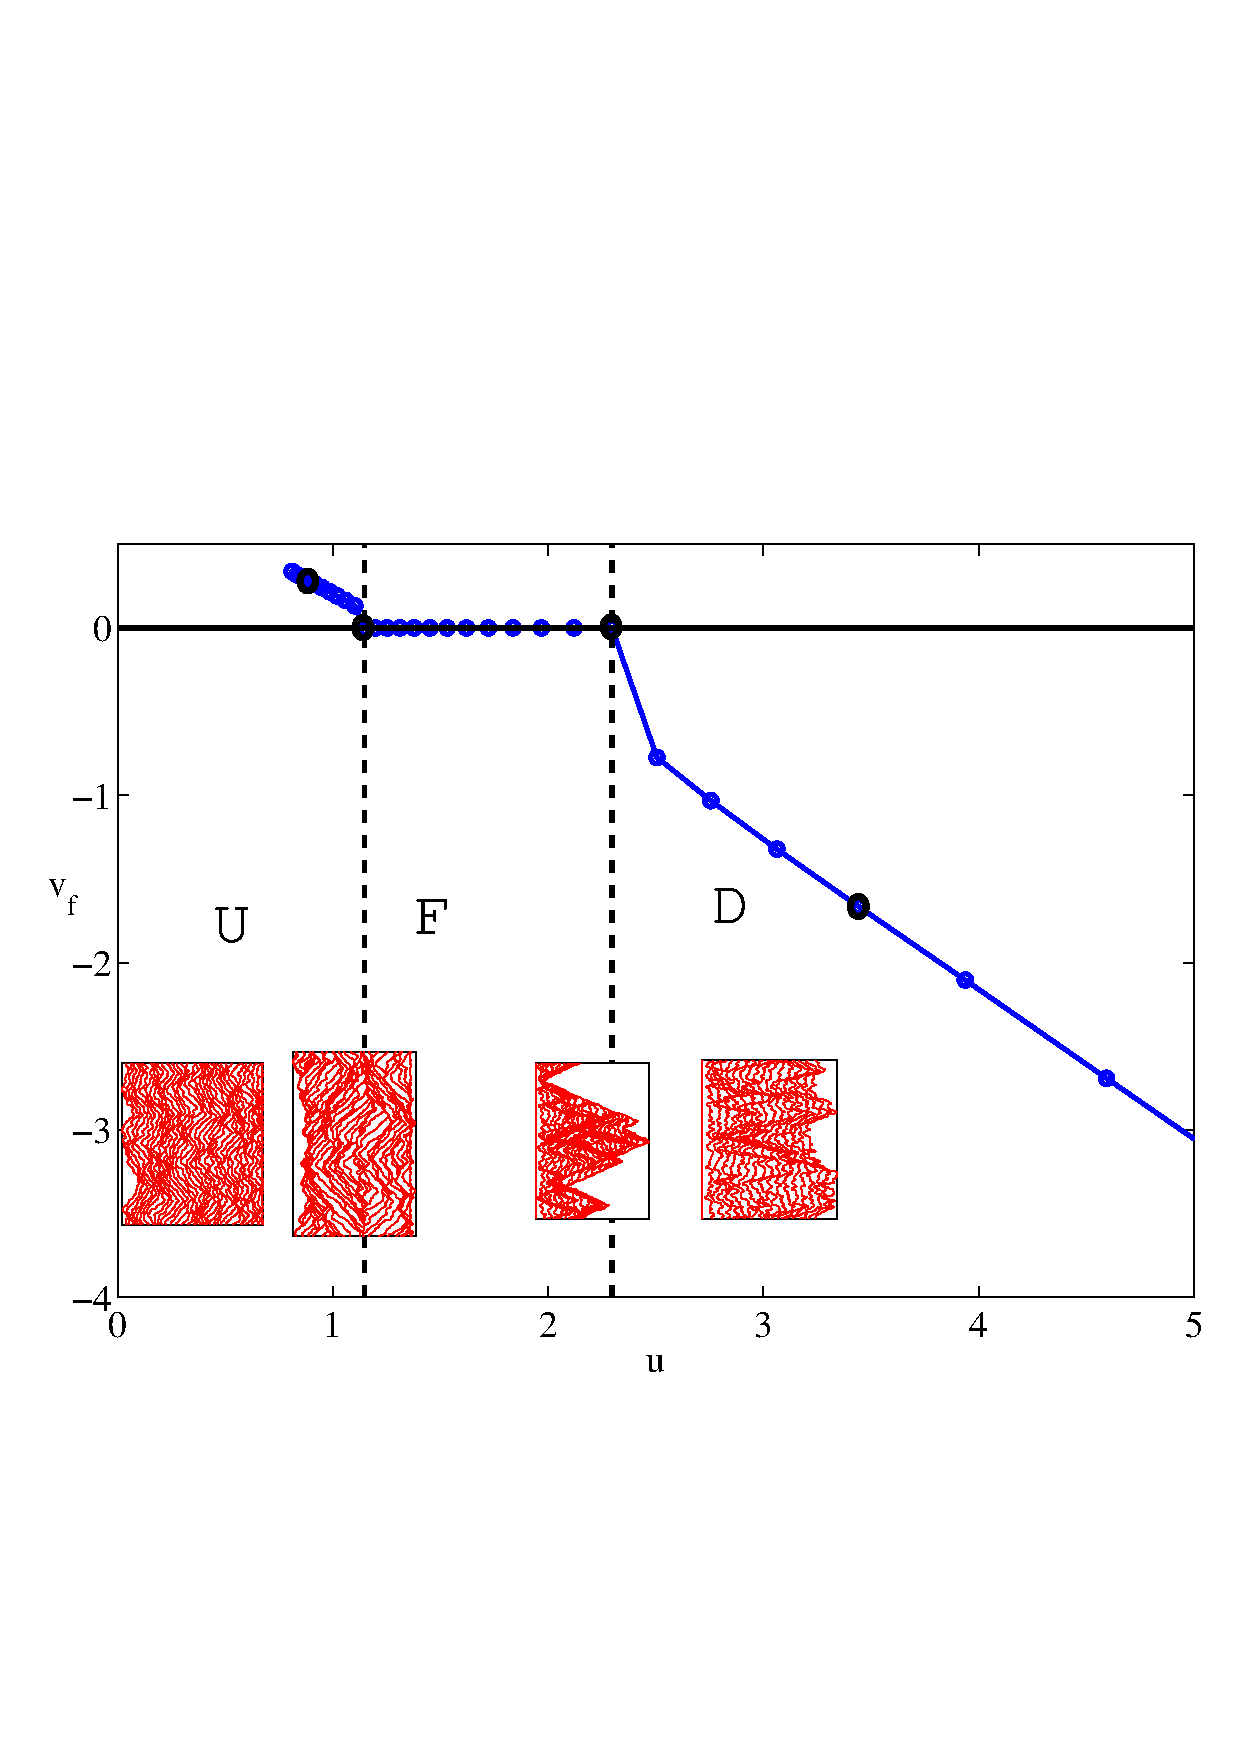
\includegraphics[width = 1.0\hsize]{\figdir/v_f_vs_v_chi_lx_0p63_sigma_0p5_laurent}
	\caption{Front velocity $v_f=V_f /V_{\chi}$ versus average flow velocity $u=-\overline{U}/V_{\chi}$ revealing the different regimes:  $U$ and  $D$ correspond respectively to a regime of front propagation upstream and downstream whereas the plateau corresponds to static, i.e. frozen fronts ($F$). $\sigma=0.5$ and $l_\chi / \lambda = 0.126 $ $\sigma=0.5$ and $l_\chi / \lambda = 0.126 $ The figures shows the evolution of the reaction front every $20,000$ time step unit in each regime.
\label{phase_diagram}}
\end{figure}


%%%%%%%%%%%%%%%%%%%%%%%%%%%%%%%%%%%%%%%%%%%%%%%%%%%%%%%%%%%%%%%%%%%%%%%%%%%%%%%%%%%%%%%%%%%%%%%%%%%%%%%%%%%%%
%%%%%%%%%%%%%%%%%%%%%%%%%%%%%%%%%%%%%%%%%%%%%%%%%%%%%%%%%%%%%%%%%%%%%%%%%%%%%%%%%%%%%%%%%%%%%%%%%%%%%%%%%%%%%
\section{Results}
Figure \ref{phase_diagram} shows the variation of the reaction front velocity $v_f$  versus the mean adverse flow velocity $u$  for $\sigma=0.5$ and $l_\chi / \lambda = 0.126 $. We observe three different regimes: For low velocities (regime $U$), the front travels upstream that is in the same direction as the chemical reaction direction ($v_f>0$).
For a range a velocities (regime $F$), the front becomes static ($v_f=0$) : this the "frozen state" plateau mentioned above. At higher velocities (regime $D$), the front travels downstream ($v_f<0$). These regimes are in agreement with the experiments \cite{atis12} as well as the typical front shapes given at the top of Fig. \ref{phase_diagram}. Interestingly, the static regime also  displays the very characteristic ``V-shape'' structure observed in experiments \cite{atis12b}.
The agreement between experiments and our model porous medium reveals that the presence of heterogeneities are able to capture the physical origin of the observed static "frozen states" plateau, eventhough the velocity distribution and correlation are different.
One of the goal of this paper is to understand the occurrence of static state and the plateau extension.
Figure \ref{lchi_sigma_eff} presents the evolution of $v_f$ versus $u$  with each of the two control parameters of the heterogeneities,  $l_{\chi}/\lambda$ and $\sigma$, while keeping the other one constant.
Figure \ref{lchi_sigma_eff}(a) shows that increasing $l_\chi/\lambda$ while keeping  $\sigma$ constant reduces the plateau width; moreover the plateau reduction occurs mainly on the side of the $F \leftrightarrow D$ transition ($FD$) whereas the $U \leftrightarrow F$ transition  ($UF$) remains almost at the same $u$ value.
 Keeping $l_\chi/\lambda$ constant and increasing the amplitude of heterogeneities (i.e. $\sigma$, Fig. \ref{lchi_sigma_eff}(b)), the plateau width increases significantly . The $FD$ transition is clearly more affected but the $UF$ transition barely too. As $\sigma$ tends to zero, that is an homogeneous porous medium, the plateau region vanishes and the velocity variations tend to the line, $v_f \approx 1-u$,  ($V_f=\overline{U}+V_{\chi}$) which is the expected behavior for an homogenous flow field leading to a simple galilean sum rule \cite{edwards02,leconte03}; in this case the front is static only for a single flow value ($u=1$). To summarize these features, Figure \ref{lchi_sigma_pred} represents the phase diagram of the different regimes as function of the two heterogeneity parameters,  $l_{\chi}/\lambda$ and $\sigma$.

\begin{figure}
\onefigure[width=0.8\hsize]{\figdir/v_f_v_chi_vs_u_mean_v_chi_var_lx_rev_lau.eps}
\onefigure[width=0.8\hsize]{\figdir/v_f_v_chi_vs_u_mean_v_chi_var_sigma_rev_lau.eps}
	\caption{Variation of plateau width versus the two heterogeneity parameters,  $l_{\chi}/\lambda$ and $\sigma$. (a) $v_f$ versus $u$ for different $l_\chi/\lambda$ keeping $\sigma=0.5$ constant. (b) $v_f$ versus $u$ for different $\sigma$ keeping $l_\chi/\lambda=0.126$ constant.  The thin lines correspond to the rough estimate of the $FD$ transition whereas the thick solid lines correspond to a more refined one (Eq. \ref{lst}). The bottom bold  almost straight lines in both figure correspond to the percolation like prediction of the $UF$ transition (see text).}
\label{lchi_sigma_eff}
\end{figure}

 \begin{figure}
% 	 \flushleft{(a)}
      \onefigure[width=0.8\hsize]{\figdir/u_stop_vs_lx_rev}
%         \flushleft{(b)}
      \onefigure[width=0.8\hsize]{\figdir/u_stop_vs_sigma_rev_lau}
	\caption{ Diagram of the observed regimes ($U$, $F$, $D$). The circles corresponds to observation of frozen fronts( $F$ : $v_f=0$) , hence the vertical give the $u$ variation of the frozen state plateau. (a) $u$ versus $l_\chi/\lambda$ at constant $\sigma=0.5$. (b) $u$ versus $\sigma$ for $l_\chi/\lambda=0.126$. The line though the data are transition lines between different regimes explained in the text.}
\label{lchi_sigma_pred}
\end{figure}

  

%%%%%%%%%%%%%%%%%%%%%%%%%%%%%%%%%%%%%%%%%%%%%%%%%%%%%%%%%%%%%%%%%%%%%%%%%%%%%%%%%%%%%%%%%%%%%%%%%%%%%%%%%%%%%
%%%%%%%%%%%%%%%%%%%%%%%%%%%%%%%%%%%%%%%%%%%%%%%%%%%%%%%%%%%%%%%%%%%%%%%%%%%%%%%%%%%%%%%%%%%%%%%%%%%%%%%%%%%%%
\section{Discussion}

In order to account for zero velocity fronts in porous media, \cite{kaern02,koptyug08} emphasize on the role  of ``excited stagnant pockets'' that would act as point source responsible for pinning spatially the front. This argument needs however to be completed: in our numerical porous medium, we do observe static fronts despite the fact that we do not have any stagnant zones. In addition this mechanism did not explain the reason why for sufficiently large velocities the front is push back again. Indeed the later has only been observed for a more complicated chemistry in combined cellular flow and mean flow \cite{schwartz08} where stagnation points are scarce. Such a plateau was observed recently experimentally in packed beads \cite{atis12,atis12b}
%It is unclear how a the stagnant pockets become unexcited again.
As we do not have stagnation points but only low velocity zones, to account for the plateau, we display on figure \ref{phase_I_to_IV} the velocity fields and front shapes for different regimes. To identify the low velocity zones, we have drawn in white the iso-contours of $U=- V_{\chi}$ where $U(x,y)$ is the local velocity. From top to bottom ($D$ to $U$ regimes), $u$ decreases and the number and the extension of white lines increases. Let us first address the $FD$ transition. It likely that the main difference between regime $D$ and $F$ (the two top figures of Fig. \ref{phase_I_to_IV}) is the presence of numerous white spots in the frozen regime where locally the mean flow is lower than the chemical velocity. We observe that the front gets pinned in these zones. Inside these spots the catalysis concentration has reached one and act as a source point or zone for its neighbors. This can also explain the V-shape structure (Fig. \ref{phase_diagram} which is the solution of the source point inside an uniform 
adverse flow \cite{atis12b}.

\begin{figure}
  \onefigure[width=0.8\hsize]{\figdir/downstream_front_casenum_1273_rev_I}
  \onefigure[width=0.8\hsize]{\figdir/downstream_front_casenum_1277_rev_I}
  \onefigure[width=0.8\hsize]{\figdir/upstream_front_casenum_1289_rev_I}
  \onefigure[width=0.8\hsize]{\figdir/upstream_front_casenum_1295_rev_I}
 \label{phase_I_to_IV}
\caption{ In grey scale, velocity field. White lines correspond to the velocity iso-contours  $U(x,y)=- V_{\chi}$ where $U(x,y)$ is the local velocity. From top to bottom, the figures correspond to the downstream regime ($D$, $u=4$), the frozen regime ($F$, $u=3$) close to the $FD$ transition,  the frozen regime ($F$, $u=1.5$) close to the $UF$ transition. Fluid is flowing from left to right whereas the chemical wave in the absence of flow would propagates from right to left. In each figure, the vertical, almost straight line corresponds to the initial front position; the jagger lines correspond to the frozen front for the $F$ regime, the ultimate position in the frame before the front get out of the medium to the right for $D$ regime and to the left for the $U$ regime.}
\end{figure}

These observation lead to a first estimate of the transition velocity $u_{FD}$ between frozen and downstream regimes.
\begin{eqnarray}
min(U(x,y)) = -V_{\chi}
\end{eqnarray}
In other words, the transition occurs when the chemical velocity becomes smaller than the global minimum of the velocity field.
This criteria has been plotted on the phase diagram Figure \ref{lchi_sigma_pred} as the thin dashed line which indeed is a larger bound over predicts the transition and does not account for the effect of $l_\chi/\lambda$.
The relevance of this later ratio can be addressed in the context of eikonal \cite{williams85} and mixing regimes \cite{edwards02,leconte04}. In the mixing regime, the front width is much larger than the characteristic length scale of the flow which in this problem is the correlation length of the permeability field $\lambda$; in such case the chemical front is sensitive to the average velocity over $l_{\chi}$ and therefore feels the average velocity field $\overline{U}$ and behaves as in an homogeneous medium leading to the above vanishing of the plateau. In the opposite eikonal thin front regime the front width is much smaller than any length scale in the system and therefore is sensitive to local velocities.
Indeed, in our simulation we are in between these two regimes but the trend is there (decreasing $l_\chi/\lambda$ leads to shorter plateau); therefore,  the finite width $l_{\chi}$ has to be taken into account in the pinning criteria. We can expect that the lower velocity zones are felt when they have a sufficiently large extension: in Fig. \ref{phase_I_to_IV}(b), we note that the front has passed through low velocity zones before being pinned. Following the determination of the contours of all the low-velocity zones, we compute the width $l_{FD}$ of each, and retain the ones with large enough size:
\begin{equation}
l_{FD}  \geq 9 l_\chi,
\label{lst}
\end{equation}
where the numerical factor ($9$) is an ad-hoc coefficient that best fits the transition.
The corresponding criteria is been plotted on Figure \ref{lchi_sigma_pred} (thick dashed line) and shows reasonable agreement for variations of both parameters.
%The evolution of the transition velocity $u_{st}$ with the two parameters can then be interpreted as the %probability to have a velocity zone weaker than the chemical reaction which as a width larger than the %chemical reaction.
Increasing $\sigma$ or increasing $\lambda/l_{\chi}$, increases naturally the probability to pin the front.\\
Even if the variation with the disorder of the transition velocity $U\leftrightarrow F$ is not very large ,
Figure \ref{phase_I_to_IV}(c-d) gives some insight of the physical mechanism at work. As $u$ is decreased, the number and the size of weak velocity zones increases. In these regions, where the flow is weaker, the front can in principle propagate upstream and then stop only when it reaches the left end-side of these zones. Consequently, we can reasonably think that one condition for the front to travel upstream is that it found a path connecting the initial front position to the left end side of the system where the flow is weaker than the chemical reaction. This is reminiscent of percolation like approach. Therefore the  $UF$ transition is likely to be determined by a path-criteria which is found using  a method analogous to the max-min algorithm \cite{hansen87}. At the transition the chemical velocity $V_{\chi }$ has to be equal to the maximum velocity found on the minimal velocity path :
$$U_{perc} = \max_{\cal C} (\min_{\cal C} U(x,y)),$$
 where $\cal C$ are pathes connecting the left-end side of the domain to the initial position of the front.
We can be briefly described the sequences used for this determination. Which consists in introducing a matrix $C_{i,j}$ defined as being the maximal velocity along all the minimal velocity pathes connecting the first column to the point $(i,j)$.

\begin{enumerate}
 \item Initialize a matrix, $C_{1,j}$ which consists of the velocity field at the inlet. ($i,j$ correspond to the $(x,y)$ coordinate respectively).
 \item At the next downstream location, $(i)$, we find $C_{min}(i,j) \equiv \min\{C_{i,j-1},C_{i,j},C_{i,j+1}\}$ for all $(j)$.
 \item Then we assign $C_{i+1,j} = \max\{C_{min}(i,j) , u_{i+1,j}\}$
 \item Repeat steps $2$ and $3$ until the other edge of the domain.
 \item $u_{perc} = \min \{C(N_x,[1,2,3...N_y])\}$ where $N_x, N_y$ are the number of points in the $x,y$ direction respectively.
\end{enumerate}
The percolation path can be found by following the reverse algorithm.
Figure \ref{perc_path} shows the percolation path corresponding to the percolation velocity for the velocity field corresponding to figure \ref{perm_vel_field}. Using the aforementioned algorithm we compute $U_{perc}$ and compare it to the observed $UF$ transition for various $l_\chi$ and $\sigma$ in figure \ref{lchi_sigma_pred}(a - b) marked by the bottom solid lines. The percolation velocity gives an accurate estimate of the critical velocity for transition from upstream regime to the frozen one. Indeed the variations with either parameter is small, the trend is there;
\begin{figure}
 \onefigure[width=0.99\hsize]{\figdir/percolation_path_casenum_1289}
        \caption{Percolation path. White and Black regions correspond respectively to $U(x,y)<u_c$ à $U(x,y)>u_c$.}
\label{perc_path}
\end{figure}
since the percolation threshold on a regular lattice is close to $1/2$, the percolation velocity satisfy $\int_{-\infty}^{u_c} pdf(u)\;du \simeq 1/2$.
It is thus expected that the critical chemical velocity is close to mean flow velocity if the probability distribution  were symetrical.
We moreover expect that the amplitude heterogeneities and its correlation has very little influence on it which is confirmed by figure \ref{lchi_sigma_pred}.
One should however recall that our flow  velocity field has a log-normal distribution and has anisotropy, which could explain that percolation is occurring for $u>1$ and the influence of $\sigma$.


One can note on Fig. \ref{perc_path} that close to percolation, higher velocity regions are also percolating to the right end side. The front is however propagating upstream because of the autocatalytic process. Whenever the reaction has managed to propagate upstream, it acts as a source of catalysis from that point and can then excited neighbors. The upstream propagation has therefore an ascendent to the downstream one.
In addition, one can note that the front is going upstream slightly before percolation. This can be explained also by the autocatalytic process: due to the fact that a low velocity cluster is ``excited'' it can excite other neighboring clusters that might spanned more upstream. Non-percolating clusters might then be exited further and further upstream.
Another mechanism could be to the finite width of the chemical front. One cluster might excite the other if the distance between the two is smaller than the chemical length.


%%%%%%%%%%%%%%%%%%%%%%%%%%%%%%%%%%%%%%%%%%%%%%%%%%%%%%%%%%%%%%%%%%%%%%%%%%%%%%%%%%%%%%%%%%%%%%%%%%%%%%%%%%%%%
%%%%%%%%%%%%%%%%%%%%%%%%%%%%%%%%%%%%%%%%%%%%%%%%%%%%%%%%%%%%%%%%%%%%%%%%%%%%%%%%%%%%%%%%%%%%%%%%%%%%%%%%%%%%%
\section{Conclusions}
Using lattice Bolzmann simulations, we have analyzed the different regimes of propagation of an autocatalytic reaction front in a heterogenous porous media when chemical reaction and flow field act in opposite directions. In agreement with previous experiments in packed beads porous media, we observe upstream, downstream fronts as well as static, frozen ones over a range of flow velocity which depends drastically on the heterogeneities of the flow field. The transition between the static regime and the downstream one is understood as due to large enough low velocity zones whereas the transition from static to upstream regime is found to be given by a kind of percolation path.




%					The bibliography
%------------------------------------------------------------------------------------------
 	\bibliographystyle{eplbib}
	\bibliography{biblio}
\end{document}
